\section{Obstacles Objective}

	\begin{frame}
		\frametitle{Robot Environment}
		\begin{columns}[T]
			\begin{column}{0.3\textwidth}
				\begin{itemize}
					\item Static obstacles location \\[1.0cm]
					\item Dynamic obstacles trajectory
				\end{itemize}
			\end{column}
			\begin{column}{0.7\textwidth}
				\centering
				\animategraphics[loop,controls,width=0.79\textwidth]{2}{pictures/robot_env_group/robot_env-}{0}{8}
				%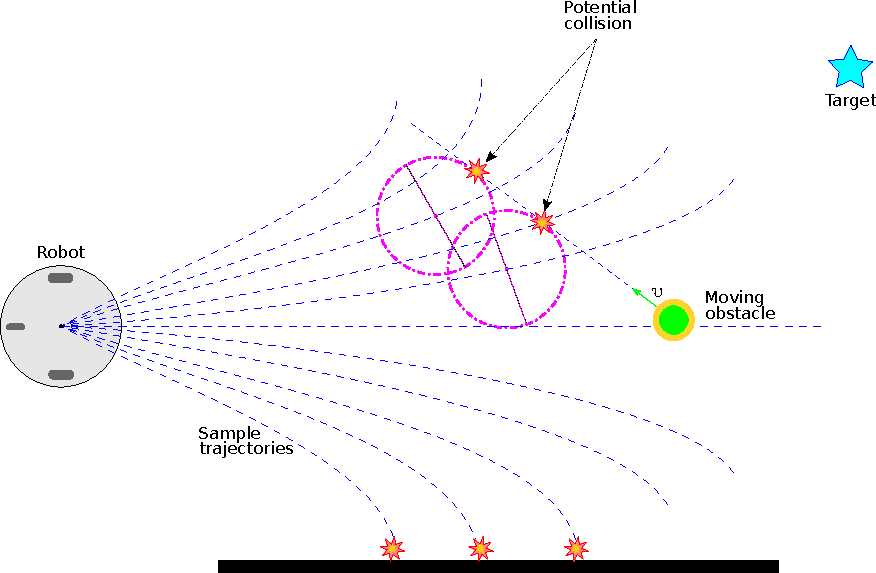
\includegraphics[scale=0.7]{pictures/robot_env.pdf}
			\end{column}
		\end{columns}
	\end{frame}

	\begin{frame}
		\frametitle{Laser Scanner}
		\begin{columns}[T]
			\begin{column}{0.42\textwidth}
				\centering
				\onslide<1->{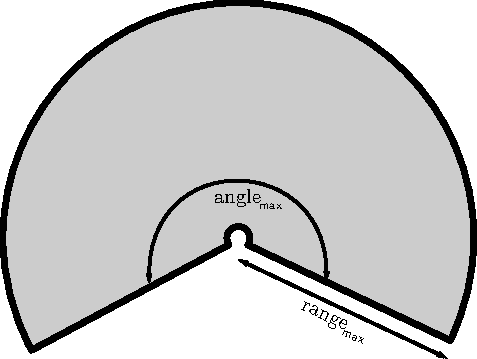
\includegraphics[scale=0.45]{pictures/laser_ranges.pdf}}
				\onslide<3->{
				\begin{block}{Laser scanner message}
					\[\overrightarrow{data}(k) = \left\{
					\begin{array}{lr}
					angle_{min} \\
					angle_{max} \\
					\overrightarrow{angle}_{inc}, \quad \qquad \forall \enspace \delta \in \overrightarrow{angle}_{inc} \\
					range_{min} \\
					range_{max} \\
					\overrightarrow{ranges}, \qquad \qquad \forall \enspace \sigma \in \overrightarrow{ranges}
					\end{array}
					\right.
					\]
				\end{block}
				}
			\end{column}
			\begin{column}{0.52\textwidth}
				\centering
				 \onslide<2->{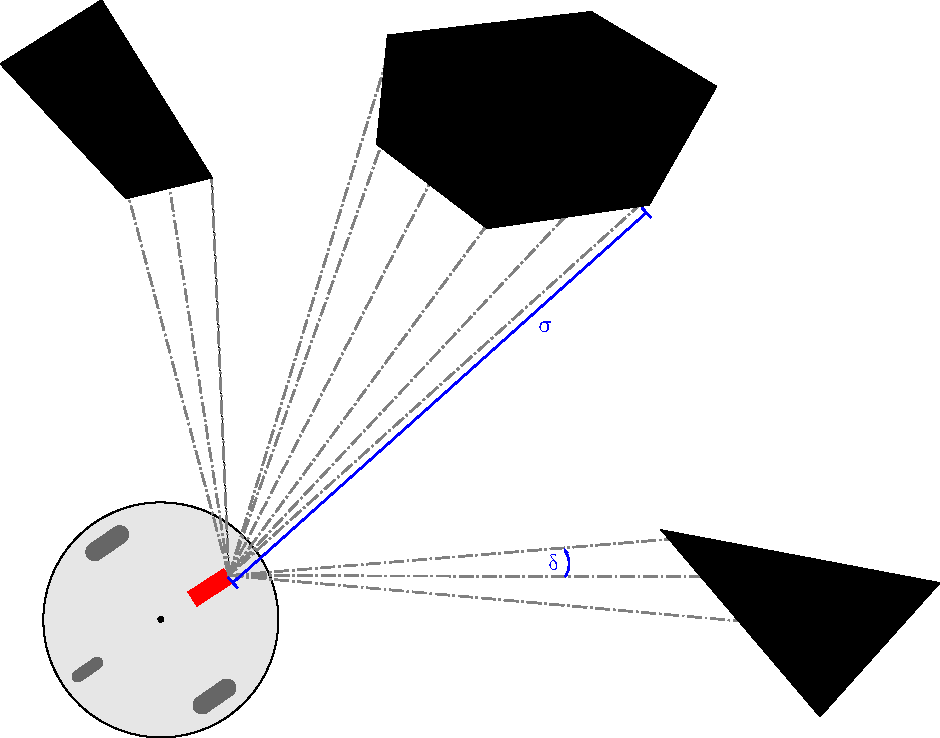
\includegraphics[scale=0.51]{pictures/robot_laser.pdf}}
			\end{column}
		\end{columns}
	\end{frame}

	\begin{frame}
		\frametitle{Homogeneous Transformation}
		\begin{columns}[T]
			\begin{column}{0.4\textwidth}
				\onslide<2->{
				\begin{block}{Rotation Matrix regarding $Z$-axis}
					\[
						T_z = 
						\begin{pmatrix}
							\cos\theta_z & -\sin\theta_z & 0 & x_{trns} \\
							\sin\theta_z &  \cos\theta_z & 0 & y_{trns}  \\
							0		   & 0 			 & 1 & z_{trns}  \\
							0		   & 0			 & 0 & 1 \\
						\end{pmatrix}
					\]
				\end{block}
				}
				\onslide<3->{
				\begin{block}{Co-ordinate Transformation}
					\[
						T_{obst\_map} = 
						T_{ft\_map} T_{r\_ft} T_{lsr\_r}
						\begin{pmatrix}
							x_{obst} \\
							y_{obst} \\
							z_{obst} \\
							1 
						\end{pmatrix}
					\]
				\end{block}
				}
			\end{column}
			\begin{column}{0.55\textwidth}
				\centering
				\onslide<1->{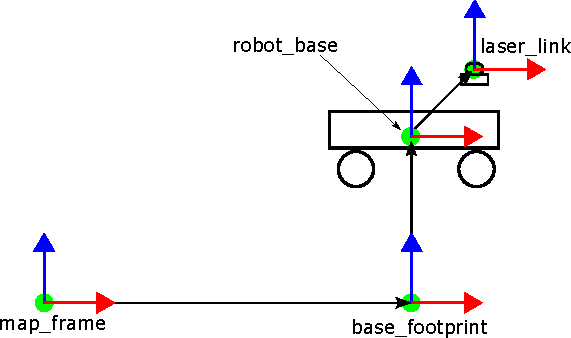
\includegraphics[scale=0.9]{pictures/laser_robot_frame.pdf}}
			\end{column}
		\end{columns}
	\end{frame}

	\begin{frame}
		\frametitle{Saved Obstacles Frame}
		\centering
		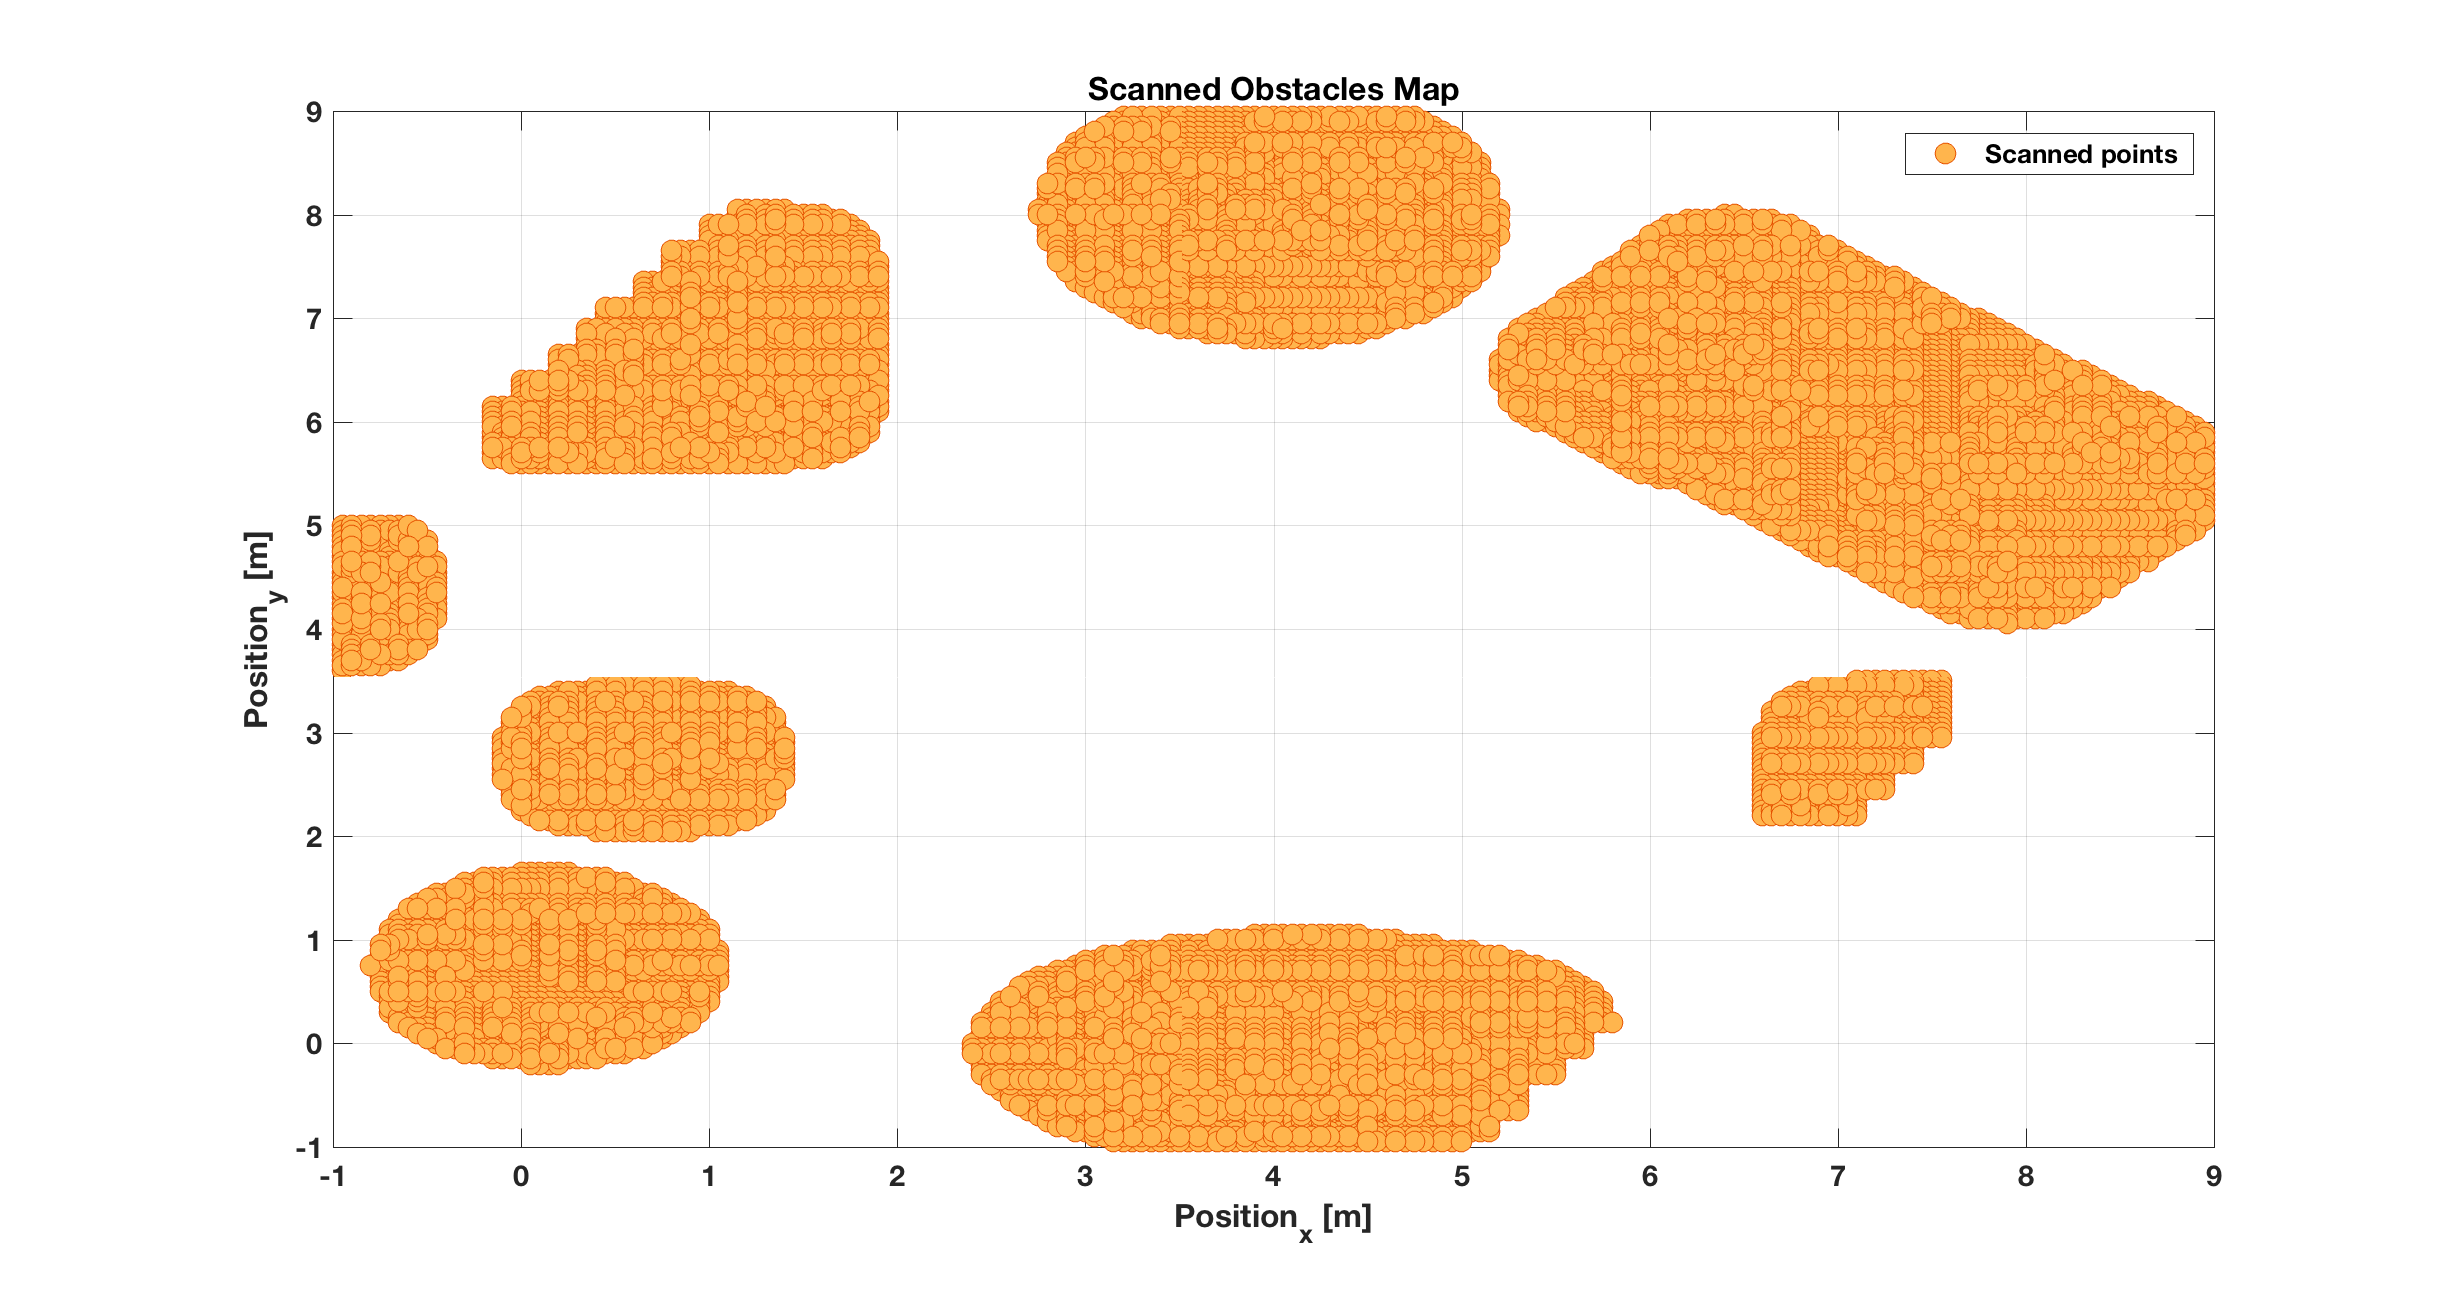
\includegraphics[scale=0.46]{pictures/intial_map.eps}
	\end{frame}

	\begin{frame}
		\onslide<1->{
		\begin{block}{Density-Based Spatial Clustering of Applications with Noise (DBSCAN) 
				\footnote[1]{Ester, M., Kriegel, H.-P., Sander, et al.
					\say{\textcolor{tudark}{A density-based algorithm for discovering clusters in large spatial databases with noise}}.}}
			Statistical search algorithm
		\end{block}
		\begin{block}{Least Square Fitting Ellipse (LSFE) 
				\footnote[2]{{Fitzgibbon, A. W., Pilu, M., and Fisher, R. B. \say{\textcolor{tudark}{Direct least squares fitting of ellipses}}.}}}
			Numerical fitting algorithm for each set of data.
		\end{block}
		}
		\begin{columns}[T]
			\onslide<2->{
			\begin{column}{0.32\textwidth}
				\begin{itemize}
					\item Edged data points
				\end{itemize}
				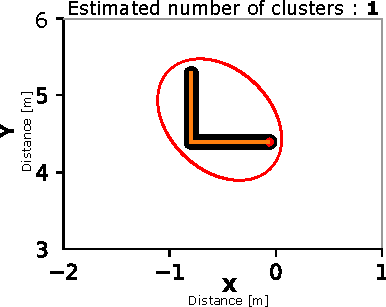
\includegraphics[scale=0.55]{pictures/lsellipse1.pdf}
			\end{column}
			}
			\onslide<3->{
			\begin{column}{0.32\textwidth}
				\begin{itemize}
					\item Concave data points
				\end{itemize}
				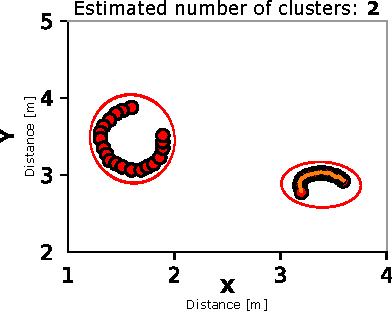
\includegraphics[scale=0.55]{pictures/lsellipse2.pdf}
			\end{column}
			}
			\onslide<4->{
			\begin{column}{0.32\textwidth}
				\begin{itemize}
					\item Lined-curved data points
				\end{itemize}
				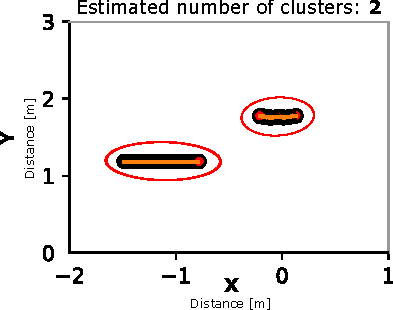
\includegraphics[scale=0.55]{pictures/lsellipse3.pdf}
			\end{column}
			}
		\end{columns}
	\end{frame}

	\begin{frame}
		\frametitle{Fitted Frame}
		\centering
		\includegraphics[scale=0.13]{pictures/map_clustered.eps}
	\end{frame}

	\begin{frame}
		\frametitle{Dynamic Obstacles Tracking 	\footnote[1]{{Redmon, J. and Farhadi, A. \say{\textcolor{tudark}{YOLO9000: better, faster, stronger}}.}}}
		\begin{columns}[T]
			\begin{column}{0.4\textwidth}
				\onslide<2->{
				\begin{block}{Dyn. obstacles estimation}
					\parbox[c][6.5\baselineskip][t]{\textwidth}{
					\begin{align*}
						&\hat{\mathbf{x}}_{i,k} = 
						\begin{pmatrix}
							\hat{x}_{i,k} \\
							\hat{y}_{i,k} \\
							\hat{\theta}_{i,k}
						\end{pmatrix},
						\qquad \qquad \hat{\mathbf{v}}_{i,k} =
						\begin{pmatrix}
							\hat{v}_{i,k} \\
							\hat{\omega}_{i,k}
						\end{pmatrix}
						\\
						&\hat{\mathbf{X}}_{i,k} := \{ \hat{\mathbf{x}}_{i,k}, \hat{\mathbf{x}}_{i,k+1}, \cdots, \hat{\mathbf{x}}_{i,k+N_p} \} \\
						&\bar{\mathbf{X}}_{i,k} := \{ \bar{\mathbf{x}}_{i,k}, \bar{\mathbf{x}}_{i,k+1}, \cdots, \bar{\mathbf{x}}_{i,k+N_p}\}
					\end{align*}
					}
				\end{block}
				}
				\onslide<3->{
				\begin{block}{Dynamic obstacles vector}
					\[
					\hat{\mathbf{Z}}_{i,k} = 
					\begin{cases}
						\hat{\mathbf{X}}_{i,k}, & \text{if } i \in I_{un} \\
						\bar{\mathbf{X}}_{i,k}, & \text{if } i \in I_{robots}.
					\end{cases}
					\]
				\end{block}
				}
			\end{column}
			\begin{column}{0.56\textwidth}
				\centering
				\onslide<1->{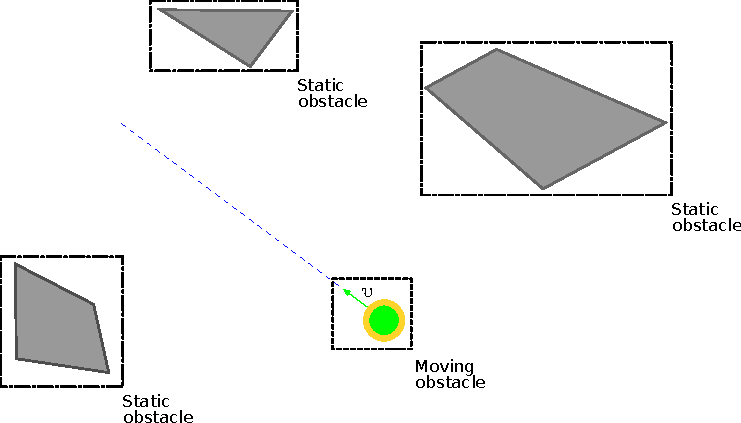
\includegraphics[scale=0.7]{pictures/robot_env_diff.pdf}}
			\end{column}
		\end{columns}
	\end{frame}

	\begin{frame}
		\frametitle{Dynamic Obstacle Estimation}
		\centering
		\movie[width=0.83\textwidth, height=0.47\textwidth]
		{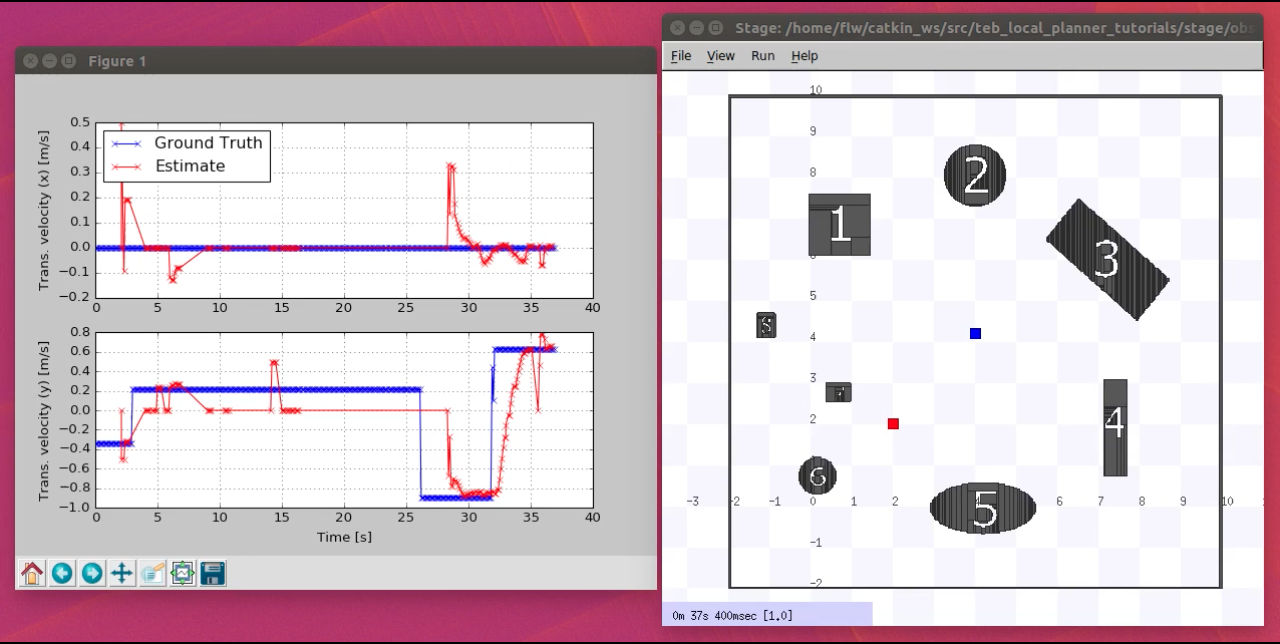
\includegraphics[width=0.83\textwidth]{pictures/kalman_filter_2.png}}{videos/klmn_best.mov}
	\end{frame}

	\begin{frame}
		\frametitle{Obstacles Detection}
		\centering
		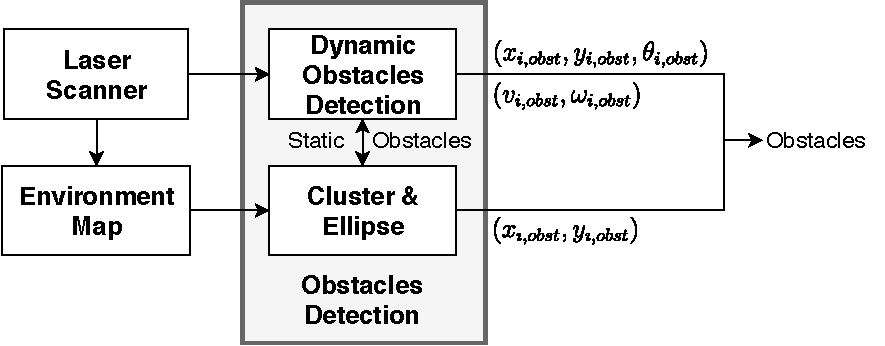
\includegraphics[scale=0.9]{pictures/block_diagram_obst_1.pdf}
	\end{frame}
